\let\negmedspace\undefined
\let\negthickspace\undefined
\documentclass[journal]{IEEEtran}
\usepackage[a5paper, margin=10mm, onecolumn]{geometry}
\usepackage{lmodern} % Ensure lmodern is loaded for pdflatex
\usepackage{tfrupee} % Include tfrupee package

\setlength{\headheight}{1cm} % Set the height of the header box
\setlength{\headsep}{0mm}     % Set the distance between the header box and the top of the text

\usepackage{gvv-book}
\usepackage{gvv}
\usepackage{cite}
\usepackage{amsmath,amssymb,amsfonts,amsthm}
\usepackage{algorithmic}
\usepackage{graphicx}
\graphicspath{{./figs/}}
\usepackage{textcomp}
\usepackage{xcolor}
\usepackage{txfonts}
\usepackage{listings}
\usepackage{enumitem}
\usepackage{mathtools}
\usepackage{gensymb}
\usepackage{comment}
\usepackage[breaklinks=true]{hyperref}
\usepackage{tkz-euclide} 
\usepackage{listings}
\usepackage{gvv}                                        
\def\inputGnumericTable{}                    
\usepackage[latin1]{inputenc}                                
\usepackage{color}                                            
\usepackage{array}                                            
\usepackage{longtable}                                       
\usepackage{calc}                            
\usepackage{multirow}                                         
\usepackage{hhline}                                          
\usepackage{ifthen}                                           
\usepackage{lscape}
\usepackage{circuitikz}

\begin{document}
	
	\bibliographystyle{IEEEtran}
	\vspace{3cm}
	
	\title{2.10.70}
	\author{EE25BTECH11042 - Nipun Dasari}
	\maketitle
	
	\renewcommand{\thefigure}{\theenumi}
	\renewcommand{\thetable}{\theenumi}
	\setlength{\intextsep}{10pt} % Space between text and floats
	
	
	\numberwithin{equation}{enumi}
	\numberwithin{figure}{enumi}
	\renewcommand{\thetable}{\theenumi}
	
	\textbf{Question}:\\
	In a $\triangle \text{ABC}$, D and E are points on $BC$ and $AC$ respectively, such that $BD = 2DC$ and $AE = 3EC$. Let P be the point of intersection of $AD$ and $BE$. Find $\frac{BP}{PE}$ using vector methods. \\ 
	\solution \\
	
	Let vertex A be the origin. The position vectors are:
	\begin{align}
		\vec{a} = \vec{0}, \quad \vec{b} = \text{Position vector of B}, \quad \vec{c} = \text{Position vector of C}
	\end{align}
	
	Position vector of point D, which divides BC in the ratio $2:1$:
	\begin{align}
		\vec{d} = \frac{1\vec{b} + 2\vec{c}}{2+1} = \frac{\vec{b} + 2\vec{c}}{3}
	\end{align}
	Position vector of point E, which divides AC in the ratio $3:1$:
	\begin{align}
		\vec{e} = \frac{1\vec{a} + 3\vec{c}}{3+1} = \frac{3\vec{c}}{4}
	\end{align}
	
	Let P divide AD in the ratio $AP:PD = \lambda:1$. The position vector of P is:
	\begin{align}
		\vec{p} = \frac{1\vec{a} + \lambda\vec{d}}{\lambda+1} = \frac{\lambda}{\lambda+1} \vec{d}
	\end{align}
	Substituting for $\vec{d}$:
	\begin{align}
		\vec{p} = \brak{ \frac{\lambda}{\lambda+1} } \brak{ \frac{\vec{b} + 2\vec{c}}{3} } = \frac{\lambda}{3\brak{\lambda+1}}\vec{b} + \frac{2\lambda}{3\brak{\lambda+1}}\vec{c} \label{eq:1}
	\end{align}
	
	Let P divide BE in the ratio $BP:PE = \mu:1$. The position vector of P is:
	\begin{align}
		\vec{p} = \frac{1\vec{b} + \mu\vec{e}}{\mu+1}
	\end{align}
	Substituting for $\vec{e}$:
	\begin{align}
		\vec{p} = \frac{1}{\mu+1}\vec{b} + \frac{\mu}{\mu+1} \vec{e} = \frac{1}{\mu+1}\vec{b} + \frac{\mu}{\mu+1} \brak{ \frac{3\vec{c}}{4} } = \frac{1}{\mu+1}\vec{b} + \frac{3\mu}{4\brak{\mu+1}}\vec{c} \label{eq:2}
	\end{align}
	
	Since $\vec{b}$ and $\vec{c}$ are non-collinear, we equate their coefficients from \eqref{eq:1} and \eqref{eq:2}.\\
	Coefficients of $\vec{b}$:
	\begin{align}
		\frac{\lambda}{3\brak{\lambda+1}} = \frac{1}{\mu+1} \label{eq:3}
	\end{align}
	Coefficients of $\vec{c}$:
	\begin{align}
		\frac{2\lambda}{3\brak{\lambda+1}} = \frac{3\mu}{4\brak{\mu+1}} \label{eq:4}
	\end{align}
	
	From \eqref{eq:3} and \eqref{eq:4}, we can see that the LHS of \eqref{eq:4} is twice the LHS of \eqref{eq:3}.
	\begin{align}
		2 \brak{\frac{1}{\mu+1}} = \frac{3\mu}{4\brak{\mu+1}}
	\end{align}
	Multiplying both sides by $4\brak{\mu+1}$:
	\begin{align}
		8 = 3\mu \implies \mu = \frac{8}{3}
	\end{align}
	The required ratio is $BP:PE = \mu:1$.
	\begin{align}
		\therefore	\frac{BP}{PE} = \mu = \frac{8}{3}
	\end{align}
	
	\begin{figure}[H]
		\centering
		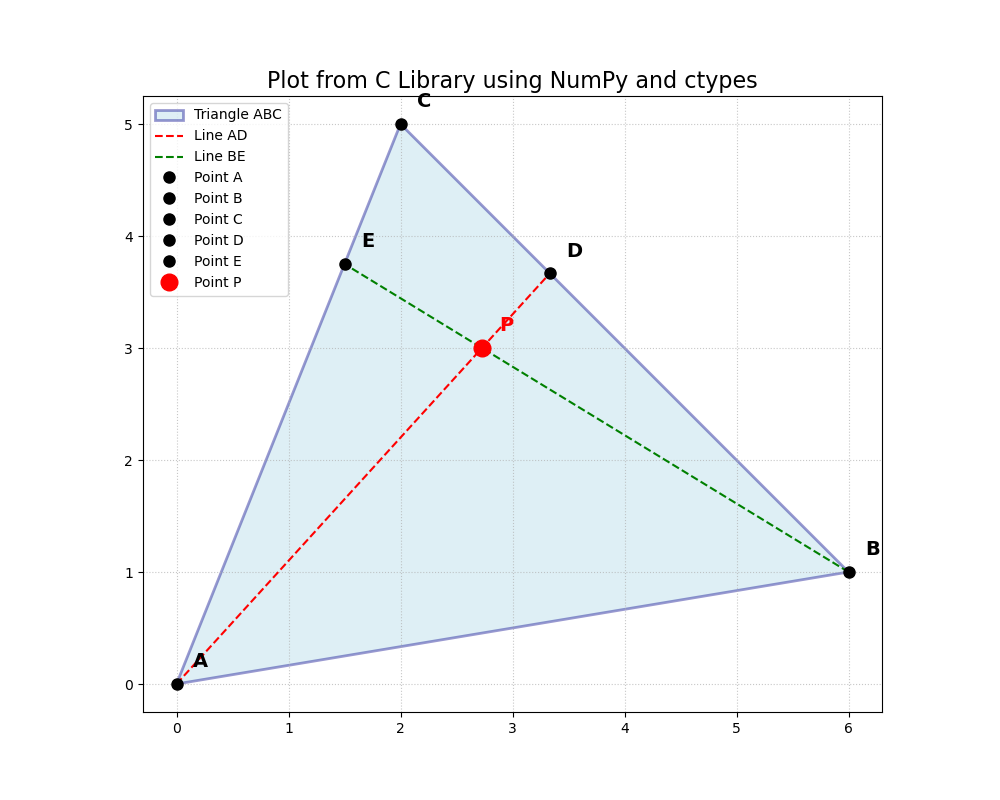
\includegraphics[width = 0.5\columnwidth]{Figure_1.png}
		\caption*{}
		\label{fig1}
	\end{figure}
		\begin{figure}[H]
		\centering
		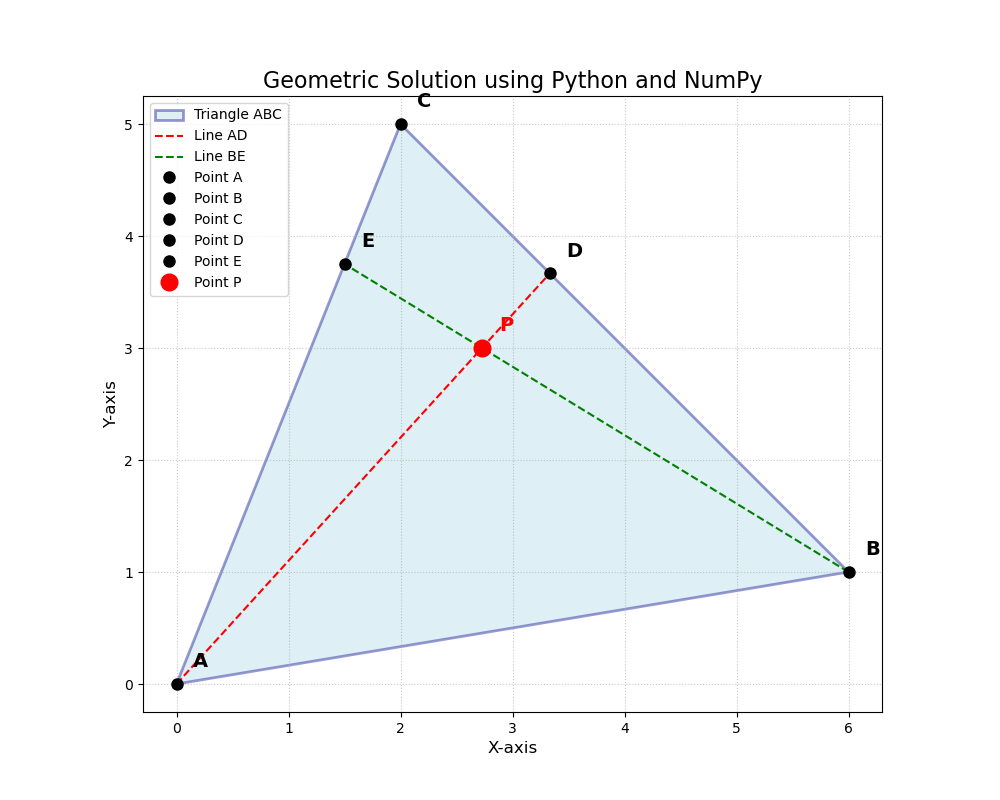
\includegraphics[width = 0.5\columnwidth]{Figure_2.png}
		\caption*{}
		\label{fig2}
	\end{figure}
	
\end{document}